\documentclass{beamer}
\usepackage[utf8]{inputenc}
\usepackage{listings}
\usepackage{multicol}
\usepackage{graphicx}


\usetheme{Frankfurt}
\usecolortheme{default}


\title[Crisis]{Introduction to contract programming}
\author{Łukasz Ziobroń}
\institute{Nokia}
\date{Code Dive Community, 2015}
\subject{Computer Science}
\lstset
{
    language=C++,
    numbers=left,
    basicstyle=\ttfamily\scriptsize,
    keywordstyle=\color{blue}\ttfamily,
    stringstyle=\color{red}\ttfamily,
    commentstyle=\color{green}\ttfamily,
}
\graphicspath{ {./img/} }
\DeclareGraphicsExtensions{.pdf,.png,.jpg}


\begin{document}


\begin{frame}
\titlepage
\end{frame}

\begin{frame}
\frametitle{Table of Contents}
\begin{multicols}{2}
\tableofcontents
\end{multicols}
\end{frame}

\section{Some examples}
\subsection{Ariane 5 mission}
\begin{frame}
\frametitle{Ariane 5 mission}
\only<1>{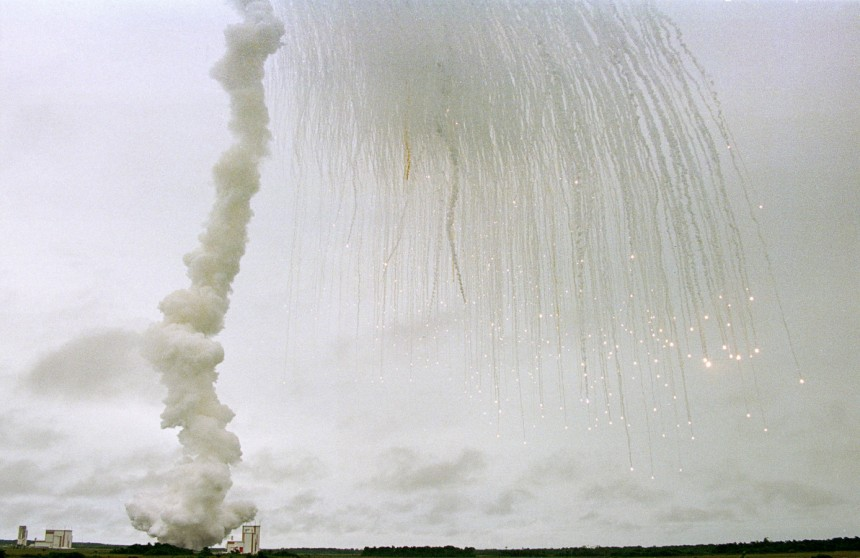
\includegraphics[scale=0.35]{ariane}}
\only<2>
{
  In 1996, the Ariane 5 rocket was reusing software from the Ariane 4. 37 seconds after its maiden launch the self-destruct safety mechanism was activated. \\~\\
  A data conversion from 64-bit floating point value to 16-bit signed integer value to be stored in a variable representing horizontal bias caused a processor trap because the floating point value was too large to be represented by a 16-bit signed integer. \footnote{https://en.wikipedia.org/wiki/Ariane\_5\#Notable\_launches} \\~\\
  This bug, existing in Ariane 4 software never came out on Ariane 4 rocket.
}
\end{frame}

\subsection{Calculator source code}
\begin{frame}[fragile]
\frametitle{Basic calculator}
\only<1>{ \lstinputlisting[linerange={26-36}]{"src/calculator.cpp"} }
\only<2>{ \lstinputlisting[linerange={38-60}]{"src/calculator.cpp"} }
\only<3>{ \lstinputlisting[linerange={62-74}]{"src/calculator.cpp"} }
\end{frame}

\subsection{Blender interface}
\begin{frame}[fragile]
\frametitle{Blender interface}
\only<1>{ \lstinputlisting[linerange={26-36}]{"src/Blender.java"} }
\end{frame}


\section{DbC Theory}
\subsection{What is a contract?}
\begin{frame}
\frametitle{What is Contract by Design?}
\setbeamercovered{transparent}
\uncover<1-2>{A paradigm which was first introduced by Bertrand Meyer, the creator of Eiffel. Although Eiffel has support for programming by contract built into the language, most of the concepts can be used in any language \footnote{http://www.cs.unc.edu/~stotts/COMP204/contract.html}.  \\~\\}
\uncover<2-2>{Basically programming by contract creates a contract between the software developer and software user - in Meyer's terms the supplier and the consumer.  \\~\\}
\end{frame}

\subsection{3 assumptions}
\begin{frame}
\frametitle{3 assumptions}
\setbeamercovered{transparent}
\uncover<1-3>{Every feature, or method, starts with a \textbf{precondition} that must be satisfied by the consumer of the routine. \\~\\}
\uncover<2-3>{And each feature ends with \textbf{postconditions} which the supplier guarantees to be true (if and only if the preconditions were met). \\~\\}
\uncover<3-3>{Also, each class has an \textbf{invariant} which must be satisfied after any changes to the object represented by the class. In the other words, the invariant guarantees the object is in a valid state.}
\end{frame}

\subsection{DbC function template}
\begin{frame}[fragile]
\frametitle{DbC function template}
\begin{lstlisting}[caption=http://www.cs.unc.edu/~stotts/COMP204/contract.html]
   SomeClass::someFunction ( AnotherClass *fillMeWithData )
   {
      // check any preconditions here
      preCondition ( fillMeWithData );   // non-NULL check

      // do your stuff to add the functionality here
      ...

      // check post conditions
      postCondition ( fillMeWithData->hasData() );  -- did we do what we said

      postCondition ( checkInvariant() );  -- class invariant check required 
                                           -- because of lack of lang support
   }
\end{lstlisting}
\end{frame}

\subsection{Let's implement the mechanism}
\begin{frame}[fragile]
\frametitle{Let's implement the mechanism}
\begin{lstlisting}
    #define  preCondition(c)     assert(c)
    #define  postCondition(c)    assert(c)
\end{lstlisting}
\begin{lstlisting}
    #define  preCondition(c)     if(!c) throw exception("preCondition c failed!")
    #define  postCondition(c)    if(!c) throw exception("Condition c failed!")
\end{lstlisting}
\end{frame}



\subsection{what is our contract}
\subsection{source code with contract}
\section{How does it work?}
\subsection{Preparsing}
\subsection{Code generation}
\subsection{example of generated code}
\section{Different languages}
\subsection{C++ - nana}
\subsection{Java - iContract}
\subsection{D - built-in mechanism}
\subsection{Eiffel - it started here}
\subsection{C++ - assertions}
\section{Some statistics}
\subsection{Code bloat - numbers}
\subsection{C++ - without, validations, contracts, generated}
\subsection{Java}

\section{Summary}
\subsection{Pros}
\begin{frame}
\frametitle{Pros}
\begin{itemize}
  \item Reduced time spent in debugger
  \item Less code
  \item Safer code
\end{itemize}
\end{frame}


\subsection{Q \& A}
\begin{frame}
\frametitle{Q \& A}
\begin{center}
\Huge Questions?

\includegraphics[scale=0.45]{dice_questions}
\end{center}
\end{frame}



\begin{frame}{Przyklad 2 kolumn}
Coś tam cośżźćł
\begin{columns}[t] % wyrownanie do gory
\column{.5\textwidth}
Tresc pierwszej kolumny
\column{.5\textwidth}
% \includegraphics[height=3cm]{rys.png}
cośisko
\end{columns}
\end{frame}

\begin{frame}
\begin{block}{To jest blok}
Jakas informacja
\end{block}

\begin{alertblock}{To jest Alert block}
Jakas wazna informacja
\end{alertblock}

\begin{exampleblock}{To jest Example block}
Jakis przyklad
\end{exampleblock}
\end{frame}


\end{document}
